\subsection{Exploratory preprocessing experiments for RQ2}
\label{app:rq2-pilot}

\subsubsection{Provenance and purpose}
The experiments documented here were implemented and executed by the Codex assistant during the project discussion, using the locally available Kaggle ASL Alphabet images. The assistant added the baseline and pilot scripts and ran the measurements. Student reproduction and the planned visual assessment remain outstanding. These results document the development of the proposed dilation experiment.

RQ2 concerns recovery of visually plausible hand landmarks among initially missed images. The measurements below establish technical recovery. The visual plausibility of all recovered configurations has yet to be assessed using a fixed rubric. N47 and other inspected pilot images should be identified as development data when constructing a subsequent evaluation set.

\subsubsection{Fresh baseline and training}
The baseline processed 78,000 original A--Z training images, comprising 3,000 images per letter. The additional classes were excluded. MediaPipe Hand Landmarker 0.10.35 ran in IMAGE mode, with a maximum of two hands and detection and presence thresholds both set to 0.50. The model file was \texttt{models/hand\_landmarker.task}. A result received \texttt{ok} when exactly one hand was returned and the project's geometric validation passed.

\begin{table}[ht]\centering
\caption{Fresh detection outcomes on original A--Z training images.}
\label{tab:rq2-baseline}
\begin{tabular}{lrr}\toprule
Outcome & Images & Percentage\\\midrule
One valid hand (\texttt{ok}) & 60,251 & 77.245\\
Zero hands (\texttt{no\_hand}) & 17,598 & 22.562\\
Multiple hands & 151 & 0.194\\
Invalid geometry & 0 & 0.000\\\midrule
Total & 78,000 & 100.000\\\bottomrule
\end{tabular}
\end{table}

A fresh SVM letter classifier was fitted to the 60,251 accepted images using 820 Shin descriptors and 15 angle features. This produced \texttt{runs/clean\_training/asl\_clean.joblib}. Its fit has no independent test score. The recovery experiments below use the pretrained MediaPipe detector; the letter classifier does not determine whether a hand is detected.

\subsubsection{N47 development example}
The original N47 image returned \texttt{no\_hand}. One application of dilation with a square \(3\times3\) kernel changed its output to \texttt{ok} at the same detector thresholds. Erosion and the tested Canny overlay retained \texttt{no\_hand}. In separate threshold probes on the original pixels, lowering only the detection threshold to 0.49 retained \texttt{no\_hand}, while 0.45 yielded \texttt{ok}. These probes show sensitivity to both preprocessing and threshold choice.

The initial N47 probes were executed as terminal commands, and their outputs were recorded in the conversation. They were not exported as a dedicated CSV. The original-versus-dilation transition was subsequently rerun when generating the example images below. The exact internal detection score was not recorded.

\begin{figure}[ht]\centering
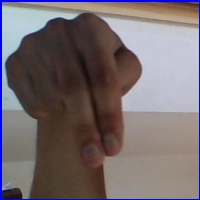
\includegraphics[height=30mm]{figures/N47_original.png}\hspace{8mm}
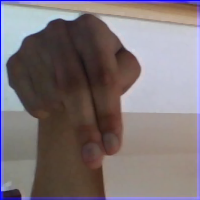
\includegraphics[height=30mm]{figures/N47_dilated.png}\hspace{8mm}
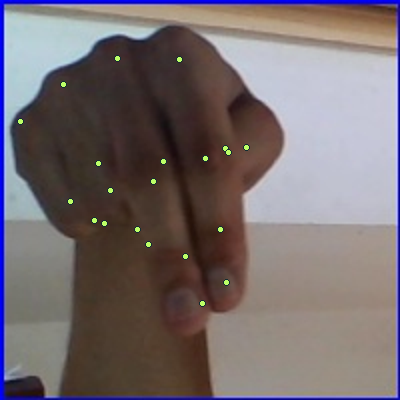
\includegraphics[height=30mm]{figures/N47_overlay.png}
\caption{N47 in its original form (left), after dilation (centre), and with recovered points overlaid on the original pixels (right). The overlay supports inspection; it does not constitute an independent landmark accuracy assessment.}
\label{fig:rq2-n47}
\end{figure}

\clearpage
\subsubsection{Letter-balanced pilot}
Using random seed 42, the pilot selected 20 initially missed and 10 initially accepted images per letter, giving 520 misses and 260 controls. The original status was rechecked before applying each transformation. Every selected photo received each of the three transformations below, with fixed detector settings.

\begin{itemize}
\item Dilation used \texttt{cv2.dilate} with a \(3\times3\) square kernel and one iteration.
\item Erosion used \texttt{cv2.erode} with the same kernel and iteration count.
\item The Canny overlay used a grayscale conversion, a \(5\times5\) Gaussian blur and Canny thresholds of 50 and 150. The three-channel edge map was added to the original RGB image with weights 0.25 and 1.0, respectively.
\end{itemize}

Image dimensions were retained, and processed arrays were supplied directly to the detector. Technical recovery means a transition from \texttt{no\_hand} to \texttt{ok}. Control loss means that an originally accepted image no longer received \texttt{ok}.

\begin{table}[ht]\centering
\caption{Exploratory pilot outcomes. Recovery denominators are 520 misses; loss denominators are 260 controls.}
\label{tab:rq2-pilot}
\begin{tabular}{lrrrr}\toprule
Transf. & Recovery & Rec (\%) & CL \footnote{Control losses} & Loss (\%)\\\midrule
Dilation & 130 & 25.00 & 6 & 2.31\\
Erosion & 64 & 12.31 & 8 & 3.08\\
Canny overlay & 49 & 9.42 & 28 & 10.77\\\bottomrule
\end{tabular}
\end{table}

The pilot gave equal weight to each letter, whereas the complete set of missed images has unequal letter counts. Its recovery percentage therefore does not directly estimate recovery across all 17,598 misses. Control losses describe applying preprocessing to already accepted images. A second-attempt procedure restricted to baseline misses bypasses these controls.

\subsubsection{Code and retained evidence}
All paths below are relative to the project root containing \texttt{app.py}.
\begin{itemize}
\item \texttt{research/data.py}, class \texttt{Detector}, defines detector settings and geometric validation.
\item \texttt{research/clean\_training.py} runs the baseline and prepares accepted inputs. The fresh classifier fit uses \texttt{--fresh-fit} in \texttt{research/live\_model.py}.
\item \texttt{research/morphology\_pilot.py} contains the transformations, deterministic sampling, paired comparisons and pilot exports.
\item \texttt{runs/clean\_training/all\_images.csv}, \texttt{no\_hand.csv} and \texttt{by\_letter.csv} contain the baseline inventory and summaries.
\item The pilot directory is \texttt{runs/clean\_training/morphology\_pilot/}. It contains \texttt{per\_foto.csv} with paired outcomes, \texttt{summary.csv} with aggregate results and \texttt{controle\_*.jpg} with overlays of recovered detections.
\end{itemize}

The pilot exports status changes and rendered overlays. A separate numerical export of all recovered landmark coordinates and a completed visual-review dataset are not yet available. The earlier \texttt{historical\_image\_audit.py} reconstructed membership in the historical accepted cohort by image ID. The fresh detector outputs listed above are the source for the present baseline counts.

\subsubsection{Reproduction and next measurement}
Run \texttt{python -m research.clean\_training --out runs/clean\_training}
from the project root with the configured Python environment. The command requires a new output directory. The existing baseline can be used to rerun \texttt{python -m research.morphology\_pilot}; this command writes to the existing pilot output paths. Preserve the original evidence before rerunning it.

A subsequent study should freeze the transformation and visual rubric, identify the development-image exclusions, and report technical and visually plausible recovery with the same eligible-image denominator. The exploratory outcomes in this appendix can motivate that design.